\chapter{Simple TSP}

%%%%%%%%%%%%%%%%%%%%%%%%%%%%%%%%%%%%%%%%%%%%%%%%%%%%%%%%%%%%%%%%%%%%%%%%%%%%%%%%%%%%%%%%%%%%%%%
\section{Introduction}

\par
In 1832, a German handbook for traveling salesmen was published, titled ''Der Handlungsreisende – wie er sein soll und was er zu tun hat, um Aufträge zu erhalten und eines glücklichen Erfolgs in seinen Geschäften gewiß zu sein – von einem alten Commis-Voyageur'' \footnote{%
	from German: ''The Traveling Salesman - how he should be and what he has to do, in order to obtain commissions and to be assured of great success in his business - by an old Commis-Voyageur''.}. 
 The book contains a definition and an elaborate description of the problem, as well as the first ever recorded reference to it as ''the Traveling Salesman Problem'', but does not give a mathematical treatment for it. 
 
\vspace{5mm}
Since then, the applications of the TSP have been found to reach far beyond travelling salesmen business. Naturally, the TSP arises in planning, transportation and logistics, problems like designing delivery routes or bus schedules are classic examples of that. There are also numerous applications in everyday life, for example for tourists wanting to visit many historical sites in a limited time, or a person running errands around town. Some other more curious and non-intuitive areas where the TSP has found applications are genetics, manufacturing, telecommunications, and neuroscience.

\vspace{5mm}
Seeing as the TSP is so widely applicable in many areas of both industrial and day-to-day life, an effective method of solution is highly desired, yet for centuries many mathematicians have struggled to find one.

\vspace{5mm}
A solution to any Traveling Salesman Problem can without a doubt be obtained by simply listing all the possible tours and selecting the best one. This would indeed always work, as every scenario with Euclidian distances will always have one or more minimal cost tours. However, it must be noted, that the number of possible tours in a TSP is $\frac{(n-1)!}{2}$, where n is the number of vertices (referred to in this work as cities). This comes from the fact that at every city the travelling salesman visits, he faces a choice of the remaining cities for his next destination, and the distance between every pair of cities is the same in each direction, forming what is called a “symmetric TSP”. Hence, for 5 cities one would find 12 possible tours, 181440 for 10 cities, 608225502004416000 for 20 and so on. For an asymmetric case, the results are even more dramatic, since the number of possible tours becomes $(n-1)!$.

\vspace{5mm}
Computing all the possible tours on a TSP becomes a huge burden, even when the problem in question is still relatively small. That is why mathematicians and computer scientists have been working on finding more efficient methods to solve the problem. Many methods have been developed, but not one of them is perfect and without drawbacks.

\vspace{5mm}
In this chapter, a small symmetric TSP consisting of only 6 cities will be solved using some of the simpler and more effective of these methods: first by applying a modified Hungarian Algorithm, then via a Binary Integer Program (BIP) in Excel. After that, the problem will be solved via the GA constructed in chapter 1. In the last section of this chapter the performance of all 3 of the methods will be discussed.




%%%%%%%%%%%%%%%%%%%%%%%%%%%%%%%%%%%%%%%%%%%%%%%%%%%%%%%%%%%%%%%%%%%%%%%%%%%%%%%%%%%%%%%%%%%%%%%
\section{The Problem}

As mentioned before, the small problem consists of 6 cities, named A to F, with the following coordinates:

\vspace{-1mm}

\begin{table}[h] 
\center
\begin{tabular}{l l l}

A (3, 0.5)   & C (6, 3.5) & E (8.5, 6) \\
B (1, 3.5)   & D (2.5, 7) &F (10, 1.5)\\

\end{tabular}
\end{table}

\vspace{-1mm}

\begin{figure}[ht] 
\centering
\vspace{-9mm}
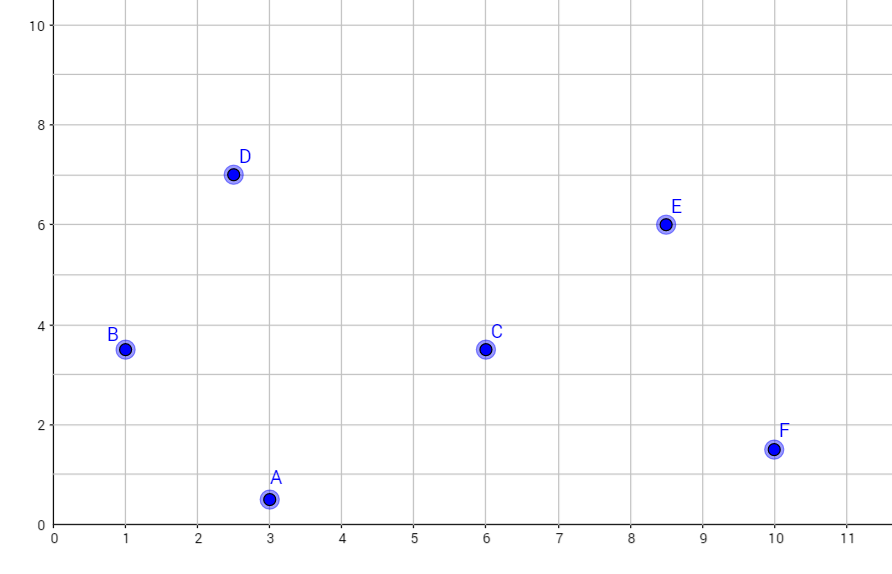
\includegraphics[height=7.5cm]{6citymap}
\caption{\textsl{6 city map}}
\label{6citymap}
\end{figure}

These can be represented on a 2-dimensional map as shown in figure \ref{6citymap}


\par
Knowing the coordinates of the points, the distance between every pair of points can be calculated, using the formula $XY=\sqrt{(x_1-y_1)^2+(x_2-y_2)^2}$  for points $X(x_1, x_2)$ and $Y(y_1, y_2)$.

\vspace{5mm}

The results can be represented as a matrix, where element in column $X$ and row $Y$ (as well as element in row $X$ and column $Y$) represents distance $XY$. For the given points A to F the matrix is shown in figure \ref{distancematrix}. In the future, it will be referred to as “the distance matrix”.

\vspace{5mm}

Note that the diagonal, which corresponds to the distance between the city and itself, is not defined, since such a tour is not allowed.

\begin{figure}[bh] 
	\centering
	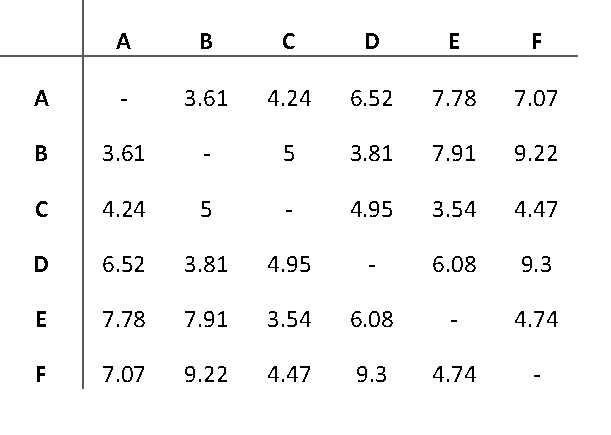
\includegraphics[height=6cm]{distancematrix}
	\caption{\textsl{The distance matrix}}
	\label{distancematrix}
\end{figure}




%%%%%%%%%%%%%%%%%%%%%%%%%%%%%%%%%%%%%%%%%%%%%%%%%%%%%%%%%%%%%%%%%%%%%%%%%%%%%%%%%%%%%%%%%%%%%%%
\section{Hungarian Algorithm}

The Hungarian Algorithm is a method designed for the assignment problem, which is a relaxation of the TSP. A modified version of it, also known as the Matrix Reduction method, or Little’s Algorithm, was introduced by John D.C. Little in 1963, in his article titled “An Algorithm For The Traveling Salesman Problem”.

\vspace{5mm}

We will now proceed to solving our 6-city problem, while simultaneously explaining the algorithm in use.

\vspace{5mm}

\underline{Step 1: Row and column reduction}
\vspace{1mm}

Begin with the distance matrix (figure \ref{distancematrix}). Identify the smallest element in every row, and subtract it from every element in that row; then do the same for every column. The resulting matrix will have a zero in each row and each column.

\vspace{5mm}

As such, the original distance matrix reduces to the following:
\vspace{3mm}


\includegraphics[height=6cm]{dmreduced}
	
	
In Little’s article, he elaborates on why this works, explaining:
\vspace{-1mm}

\begin{displayquote} 
''If a constant is subtracted from each element of the first row (of the distance matrix), that constant is subtracted from the cost of every tour. This is because every tour must include one and only one element from the first row. The relative costs of all tours, however, are unchanged and so the tour which would be optimal is unchanged. The same argument can be applied to the columns.	''
\end{displayquote}
	
	
\underline{Step 2: Penalty calculation}	
\vspace{1mm}
	
For each zero in the new matrix note the sum between the minimum element in the row and the minimum element in the column of that zero (omitting the zero itself). That number is called the penalty associated with the zero.

\vspace{5mm}

Therefore, the penalty associated with the zero in position AB is 0.63, since the smallest element in row A is 0.63, and smallest element in column B is 0. Similarly, the penalty of the zero in position BD is 1.21, and so on. The complete matrix displaying all the penalties is shown in the figure below:	
\vspace{3mm}
	
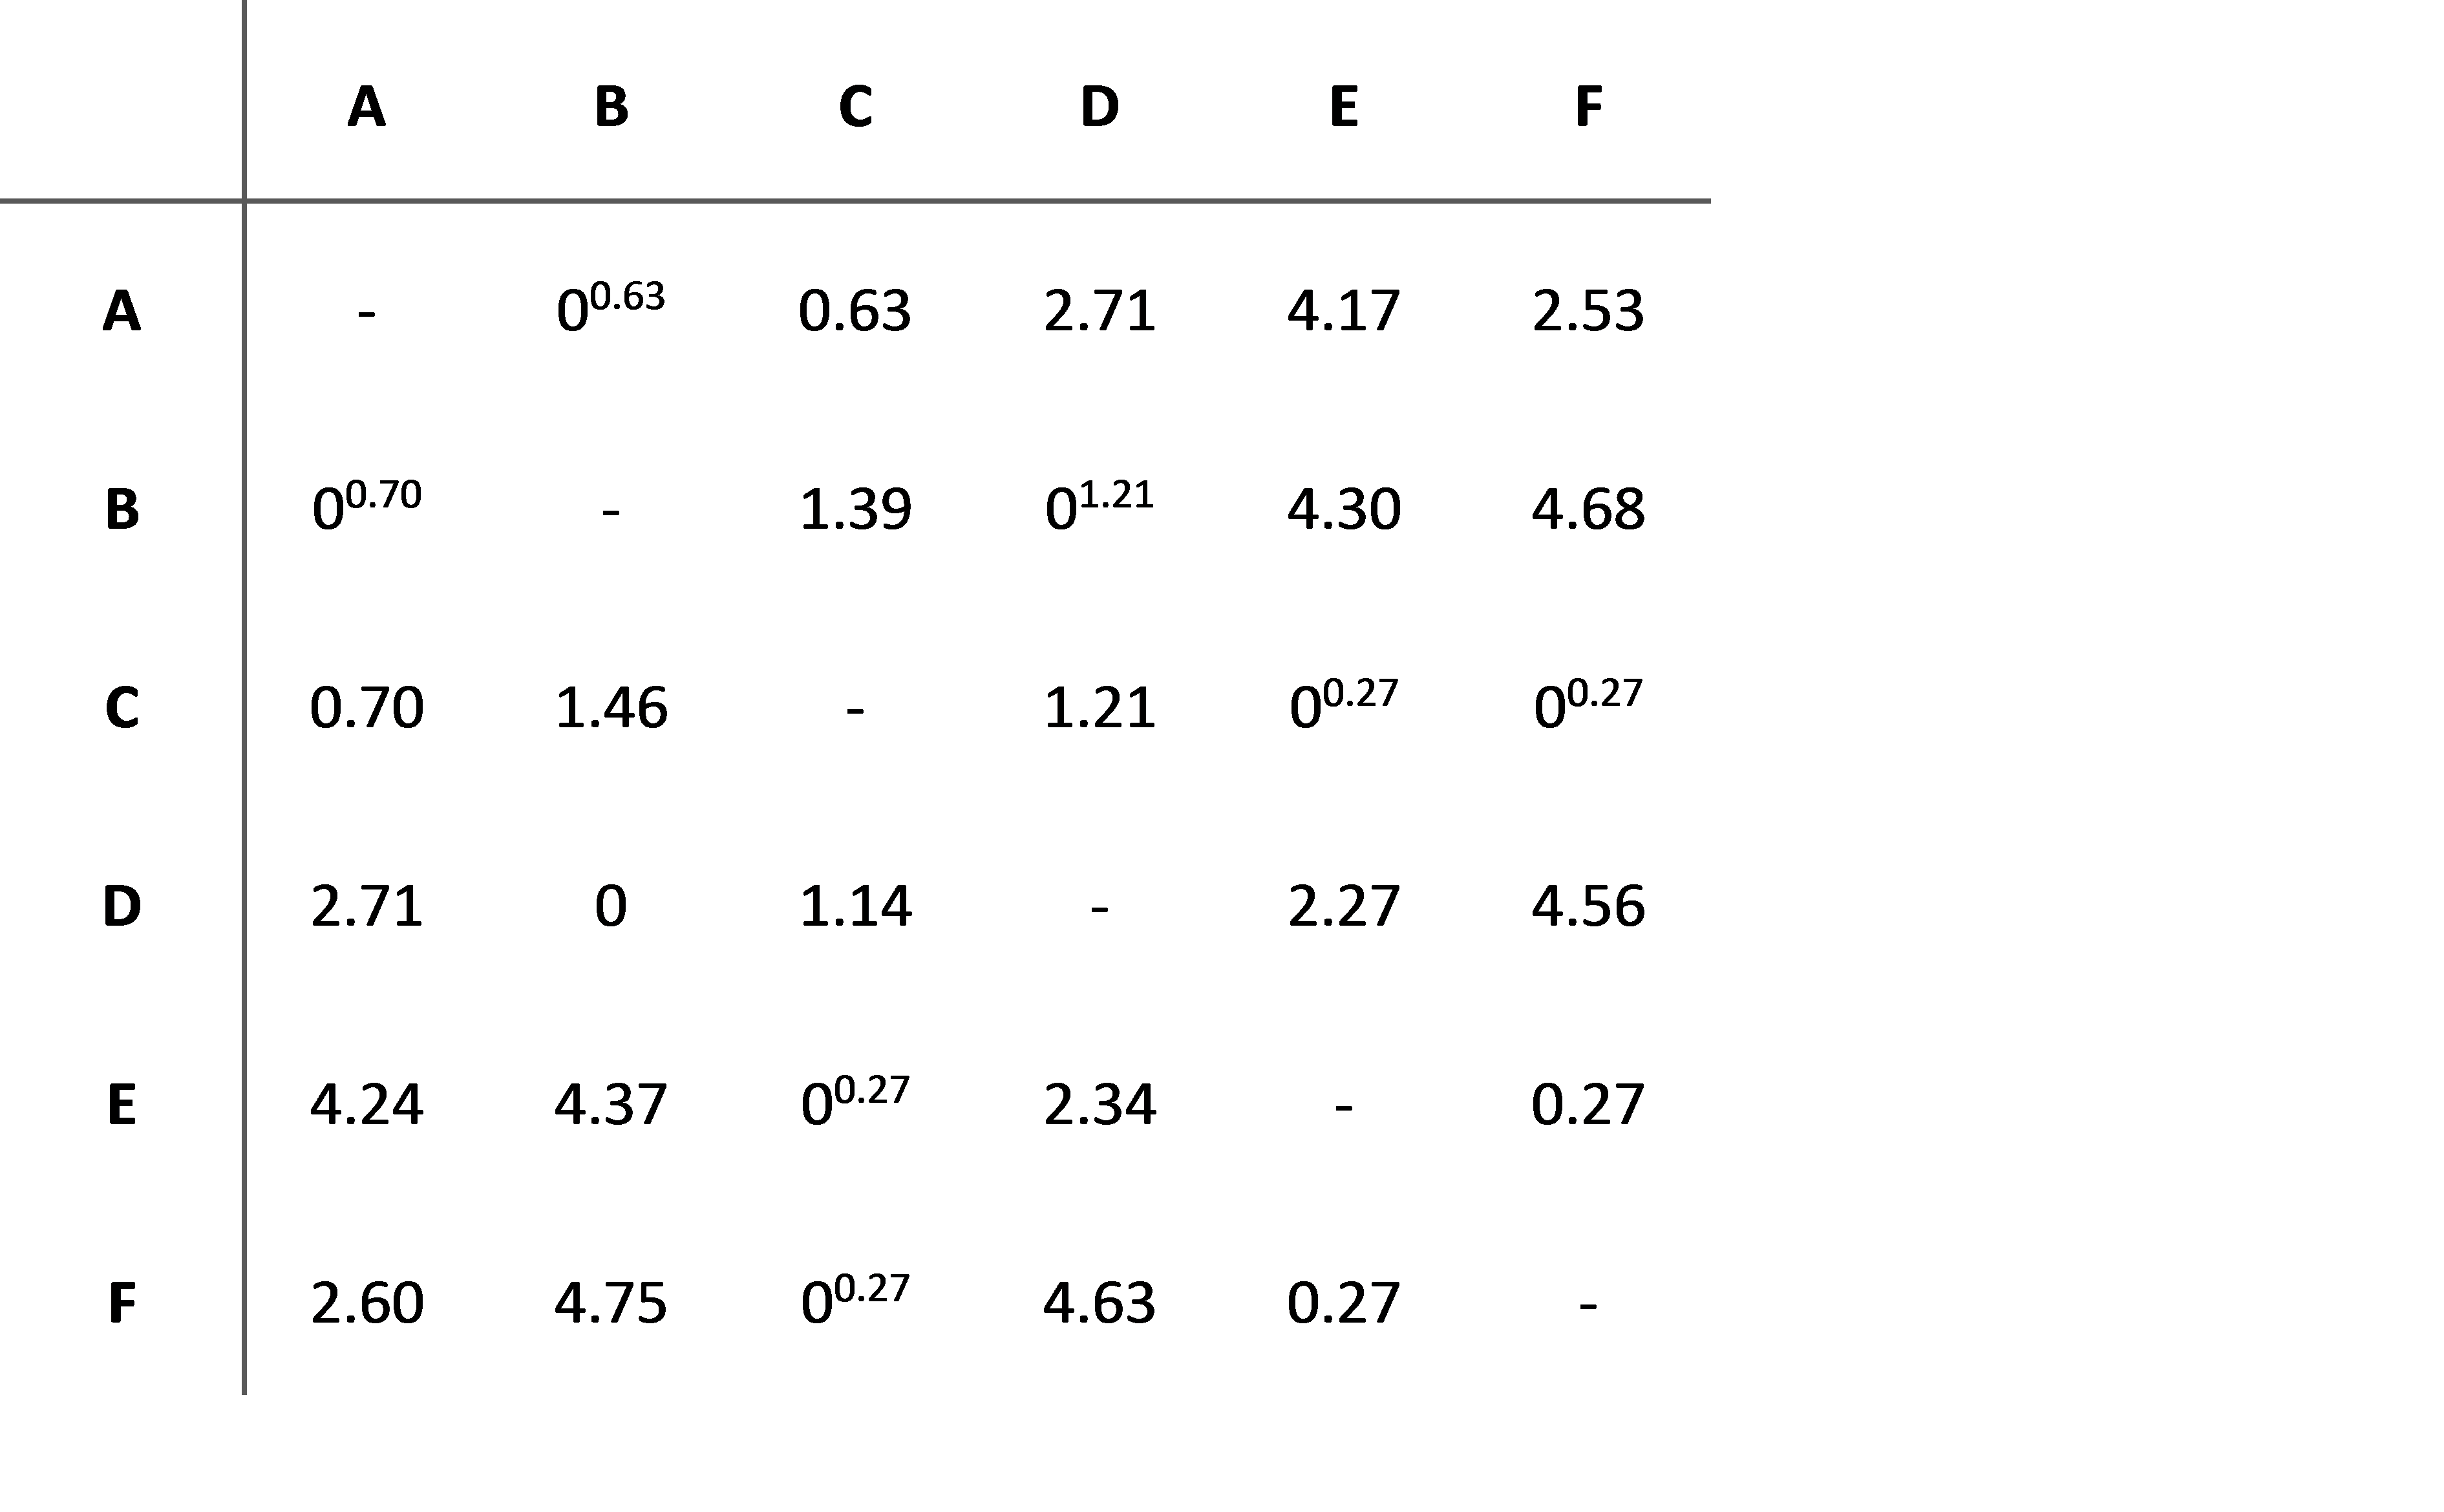
\includegraphics[height=6cm]{dmpenalties}
	
It is interesting to note, that although Little’s work describes the same process, it doesn’t refer to those numbers as “the penalties".

\vspace{5mm}

\underline{Step 3: Row and column elimination}
\vspace{1mm}

Select the zero with the highest penalty. If there is more than one zero with the same penalty, select arbitrarily. The row and column of that zero can be eliminated from the matrix, and its position noted down as part of the optimum tour.

\vspace{5mm}

In our case the zero in position BD has the highest penalty. Therefore, BD is the first definitive road in the final optimum tour that we are working towards. Hence it can be eliminated from the matrix:

\vspace{3mm}

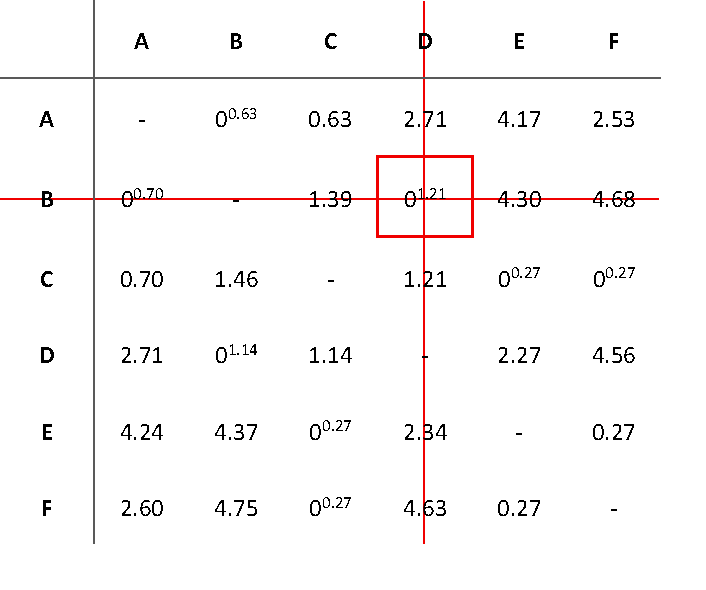
\includegraphics[height=6cm]{dmelimination} \hspace{5mm}  
\includegraphics[height=5.2cm]{dmlast}


\vspace{5mm}

\underline{Step 4: Repeat steps 1 to 3}
\vspace{1mm}

For the new matrix, repeat all the steps from the beginning: first row and column reduction, then penalty calculation, and row and column elimination, until reaching a 2x2 matrix. If no mistakes have been made, 3 elements will be zeros with penalty of zero, and the remaining element undefined. In such a matrix, only two roads are possible, and they will be the last entries on the list of roads, forming a complete tour.

\vspace{5mm}

Our 6-city problem eventually reduces to the following 2x2 matrix:
\vspace{3cm}

%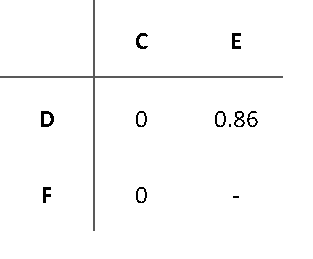
\includegraphics[height=2.5cm]{2x2matrix}

With the following assignments already made:
\par B $\rightarrow$ D, 
\par A $\rightarrow$ B, 
\par C $\rightarrow$ A, 
\par E $\rightarrow$ F.

\vspace{3mm}

The full step-by-step process can be seen in the appendix *** %\ref{appendix2}

\vspace{5mm}

We complete this list by selecting assignments F $\rightarrow$ C and D $\rightarrow$ E from figure *** %\ref{2x2matrix}
which gives us the following tour:

\vspace{2mm}

A $\rightarrow$ B $\rightarrow$ D $\rightarrow$ E $\rightarrow$ F $\rightarrow$ C $\rightarrow$ A


\begin{figure}[ht] 
	\centering
	\vspace{-9mm}
	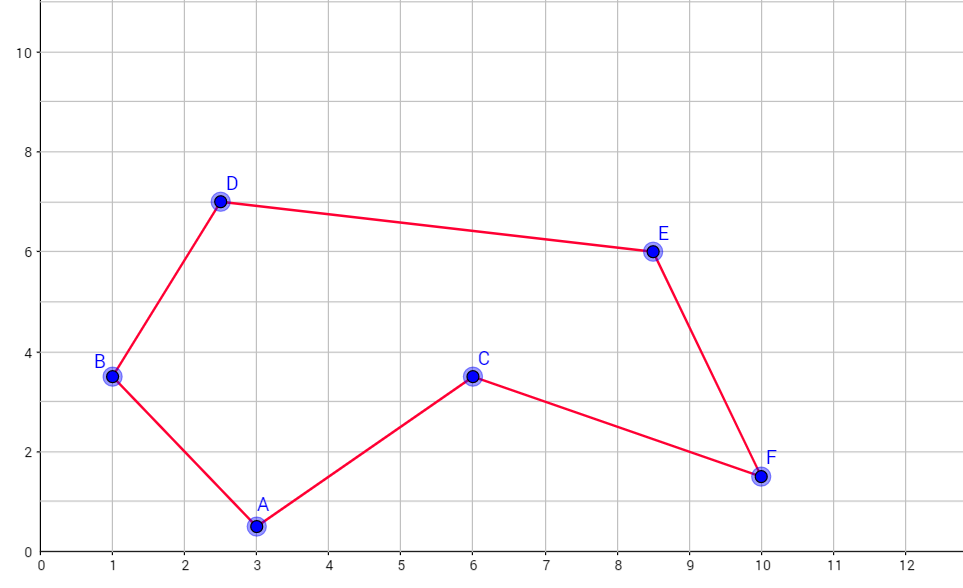
\includegraphics[height=7.5cm]{6citytour}
	\caption{\textsl{Final tour}}
	\label{6citytour}
\end{figure}

Looking back at the distance matrix (figure \ref{distancematrix}), the total distance of this tour is 26.95




%%%%%%%%%%%%%%%%%%%%%%%%%%%%%%%%%%%%%%%%%%%%%%%%%%%%%%%%%%%%%%%%%%%%%%%%%%%%%%%%%%%%%%%%%%%%%%%
\section{Binary Integer Program}

The optimum TSP tour can also be determined using a Binary Integer Program (BIP) formulation of the problem.

\vspace{5mm}

Let $x_{ij}$ be the distance between cities $i$ and $j$, given by the distance matrix in figure \ref{distancematrix} and let $y_{ij}$ be the binary decision variable, s.t.

\[
y_{ij}= 
\begin{cases}
1, & \text{if road $ij$ is part of the tour}\\
0 & \text{otherwise}
\end{cases}
\]
	

\vspace{5mm}
Then, the BIP formulation of the TSP is:
\vspace{5mm}	

Minimize

\vspace{-3mm}	
\begin{center}
$z = \sum_{i} \sum_{j} x_{ij}y_{ij}$
\end{center}	 

such that
\vspace{-3mm}	
\begin{center}
	\sum_{i} $y_{ij}=1$ for all $j$,
	
	\sum_{j} $y_{ij}$=1 for all $i$,
	
	And $y_{ij}$ binary for all $i$, $j$.
\end{center}	
	
	
This can be implemented into Excel and solved using the Solver function.
\vspace{5mm}

Since nowhere in the current formulation of the problem there is a constraint that requires the solution to be one single connected tour, it is highly likely that the solution will contain subtours. However, the TSP does not allow for subtours, so they need to be eliminated with additional constraints.
\vspace{5mm}

Using the distance matrix from figure \ref{distancematrix} for the $x_{ij}$ values, and after manually eliminating all subtours, the BIP gives the solution $z=26.95$, which tour A $\rightarrow$ B $\rightarrow$ D $\rightarrow$ E $\rightarrow$ F $\rightarrow$ C $\rightarrow$ A, which is the same result as the one obtained via the Hungarian Algorithm in section 2.3
	
	
	
	
%%%%%%%%%%%%%%%%%%%%%%%%%%%%%%%%%%%%%%%%%%%%%%%%%%%%%%%%%%%%%%%%%%%%%%%%%%%%%%%%%%%%%%%%%%%%%%%
\section{Genetic Algorithm}	
	
Given the distance matrix in figure \ref{distancematrix}, a reasonable poolsize and generation number, for example 200 and 1000 respectively, the GA is able to find the same solution for the problem as the BIP and the Hungarian Algorithm every time.



%%%%%%%%%%%%%%%%%%%%%%%%%%%%%%%%%%%%%%%%%%%%%%%%%%%%%%%%%%%%%%%%%%%%%%%%%%%%%%%%%%%%%%%%%%%%%%%
\section{Performance Evaluation}	
	
When looking at the efficiency of methods, the main factor to consider is the time taken to reach the optimum solution. In the case of the TSP, an optimum is not always possible, so it is sensible to consider just a reasonable solution. Luckily, with this problem, all 3 methods in question give the optimum solution.

\vspace{5mm}

Solving a TSP with the Hungarian algorithm takes a substantial amount of time, especially if it is done by hand. This is due to the fact that every newly reduced matrix has to be re-written every time to perform the next step (see appendix 2). Additionally, manual computations are very prone mistakes and miscalculations. As such, for the simple TSP it took a total of 2 hours to reach the optimum solution, excluding the 40 minutes it took to manually construct the distance matrix. This is a colossal amount of time, considering the problem consists of only 6 cities. Arguably, it could’ve taken less time to approach it with brute force: list all the tours and select the lowest one.

\vspace{5mm}

The Binary Integer Program, done in Excel, found that same solution in 2 seconds, but the preparations took approximately 30 minutes. These include formulating the problem with initial constraints and adding extra subtour elimination constraints where necessary.

\vspace{5mm}

The GA found the solution to this problem in under 2 seconds, which suggests that it is most efficient. However, the process of writing the program is by far the longest, spreading over several days, indicating that the GA is actually the most inefficient out of the 3 methods.

\vspace{5mm}

It must be noted that these values are not an objective measure of the efficiency of the methods. Surely, for each of the methods there are ways to decrease the time. For example, if the Hungarian Algorithm is not done manually, but rather programed on a computer, a significant amount of time can be saved, since the computer does calculations faster and does not make mistakes, or if the Genetic Algorithm is written by an expert, it may only require several hours of work, rather than several days. Therefore, the values give above are superficial and should not be taken as an accurate measure of efficiency, but rather a mere representation.

\vspace{5mm}

From this, the conclusion can be made, that in the case of a relatively small problem and easy access to a computer (with Excel-solver), the most efficient method is the BIP. However, as the problem gets larger, Excel-solver becomes insufficient, as it accepts only a limited number of variables. When that threshold is exceeded, the GA becomes most efficient. Additionally, if there is a large number of problems, the GA is more efficient than the BIP as well, because the same GA can work on any TSP, whereas a BIP needs a change of constraints for every individual one. The Hungarian Algorithm is never efficient, unless no computer is available for use.